\documentclass[a4paper,12pt]{article} 



%Добавляет возможность искать и копировать текст
\usepackage{cmap}

%Убирает пробел между названием таблицы/рисунка и самой таблицей/рисунком
\usepackage{caption}
\captionsetup[table]{skip= -0 cm}
\captionsetup[figure]{skip= -0 cm}

%Выравнивание названия таблиц по левому краю
%\usepackage[nooneline]{caption} 
%Размеры отступов 
\usepackage[left=20mm, top=20mm, right=20mm, bottom=20mm, footskip=10mm]{geometry}

%Рисунки
\usepackage{graphicx}
\usepackage{wrapfig} %обтекание элементов
\graphicspath{{graphs}{figures}}  % папки с картинками

%Русский язык в формулах
%\usepackage{mathtext}

%  Русский язык
\usepackage[T2A]{fontenc}			
\usepackage[utf8]{inputenc}			
\usepackage[english,russian]{babel}	

%Готические буквы
\usepackage{amssymb}

% Математика
\usepackage{amsmath,amsfonts,amssymb,amsthm,mathtools} 
\usepackage{wasysym}

%Цветные подписи в таблице
\usepackage[table,xcdraw]{xcolor}

\usepackage{fancyhdr} % Колонтитулы
 	\pagestyle{fancy}
 	\renewcommand{\headrulewidth}{0.3mm}  % Толщина линейки, отчеркивающей верхний колонтитул
 	%\lfoot{Нижний левый}
 	%\rfoot{Нижний правый}
 	\rhead{Кафедра вакуумной электроники}
 	%\chead{Верхний в центре}
 	\lhead{Диод Шоттки}
 	% \cfoot{Нижний в центре} % По умолчанию здесь номер страницы
 	
\begin{document} 

%Титульник 
\begin{titlepage}
	\begin{center}
		\large 	МИНИСТЕРСТВО ОБРАЗОВАНИЯ И НАУКИ РОССИЙСКОЙ ФЕДЕРАЦИИ\\
				МОСКОВСКИЙ ФИЗИКО-ТЕХНИЧЕСКИЙ ИНСТИТУТ \\
				(НАЦИОНАЛЬНЫЙ ИССЛЕДОВАТЕЛЬСКИЙ ИНСТИТУТ)\\ 
				ФИЗТЕХ-ШКОЛА ЭЛЕКТРОНИКИ, ФОТОНИКИ \\
				И МОЛЕКУЛЯРНОЙ ФИЗИКИ \\
		
		
		\vspace{4.0 cm}
		\LARGE{Кафедра вакуумной электроники \\ 
		Отчет по лабораторной работе} \\ 
		\LARGE \textbf{Диод Шоттки} \\
	\end{center}
	\vspace{3 cm} \large

	%Надо подумать как это нормально написать	
	\begin{flushleft}
		Работу выполнили \hspace{5.5cm}  \underline{\hspace{3cm}} А.И.Белостоцкий \\	
		\hspace{9.8cm}  \underline{\hspace{3cm}} Д.Е.Вовк \\
		\hspace{9.8cm}  \underline{\hspace{3cm}} Е.Ионидис \\
		\hspace{9.8cm}  \underline{\hspace{3cm}} С.Розенталь \\
		\vspace{2cm}
		Работу принял, оценка \hspace{4.3cm} \underline{\hspace{3cm}}
	\end{flushleft}
	
	
	\vfill

	\begin{center}
	Долгопрудный, 2021 г.
	\end{center}
\end{titlepage}                                                                      

\tableofcontents

\newpage

\section{Аннотация}
В данной работе изучается изготовление и принципы работы диода Шоттки. Диод представляет собой часть пластины из pSi, на которую был напылен тонкий слой Au -- для омического контакта и Al -- для контакта Шоттки. Исследуются вольтамперные характеристики изготовленных образцов.

\section{Применение диодов Шоттки}

Диоды Шоттки имеют достаточно широкое применение в современной жизни, в особенности в приборах, где требуется минимальное прямое падение напряжения. Чаще всего диод
Шоттки можно встретить в компьютерных блоках питания, а также в импульсивных стабилизаторах напряжения. Помимо этого, диод Шоттки можно увидеть в таких приборах,
как приемники альфа и бета излучения, детекторы нейтронного излучения и солнечные
батареи.

\section{Процесс изготовления}

\subsection{Напыление слоя металла}
Для изготовления диода необходимо было напылить на пластину из pSi тонкий слой -- 300 нм -- алюминия и золота. Напыление проводилось на установках MEB 550S и Nanomaster NEE-4000, используя метод электронно-лучевого напыления.

\begin{minipage}{.49\textwidth}
  \begin{center}
 	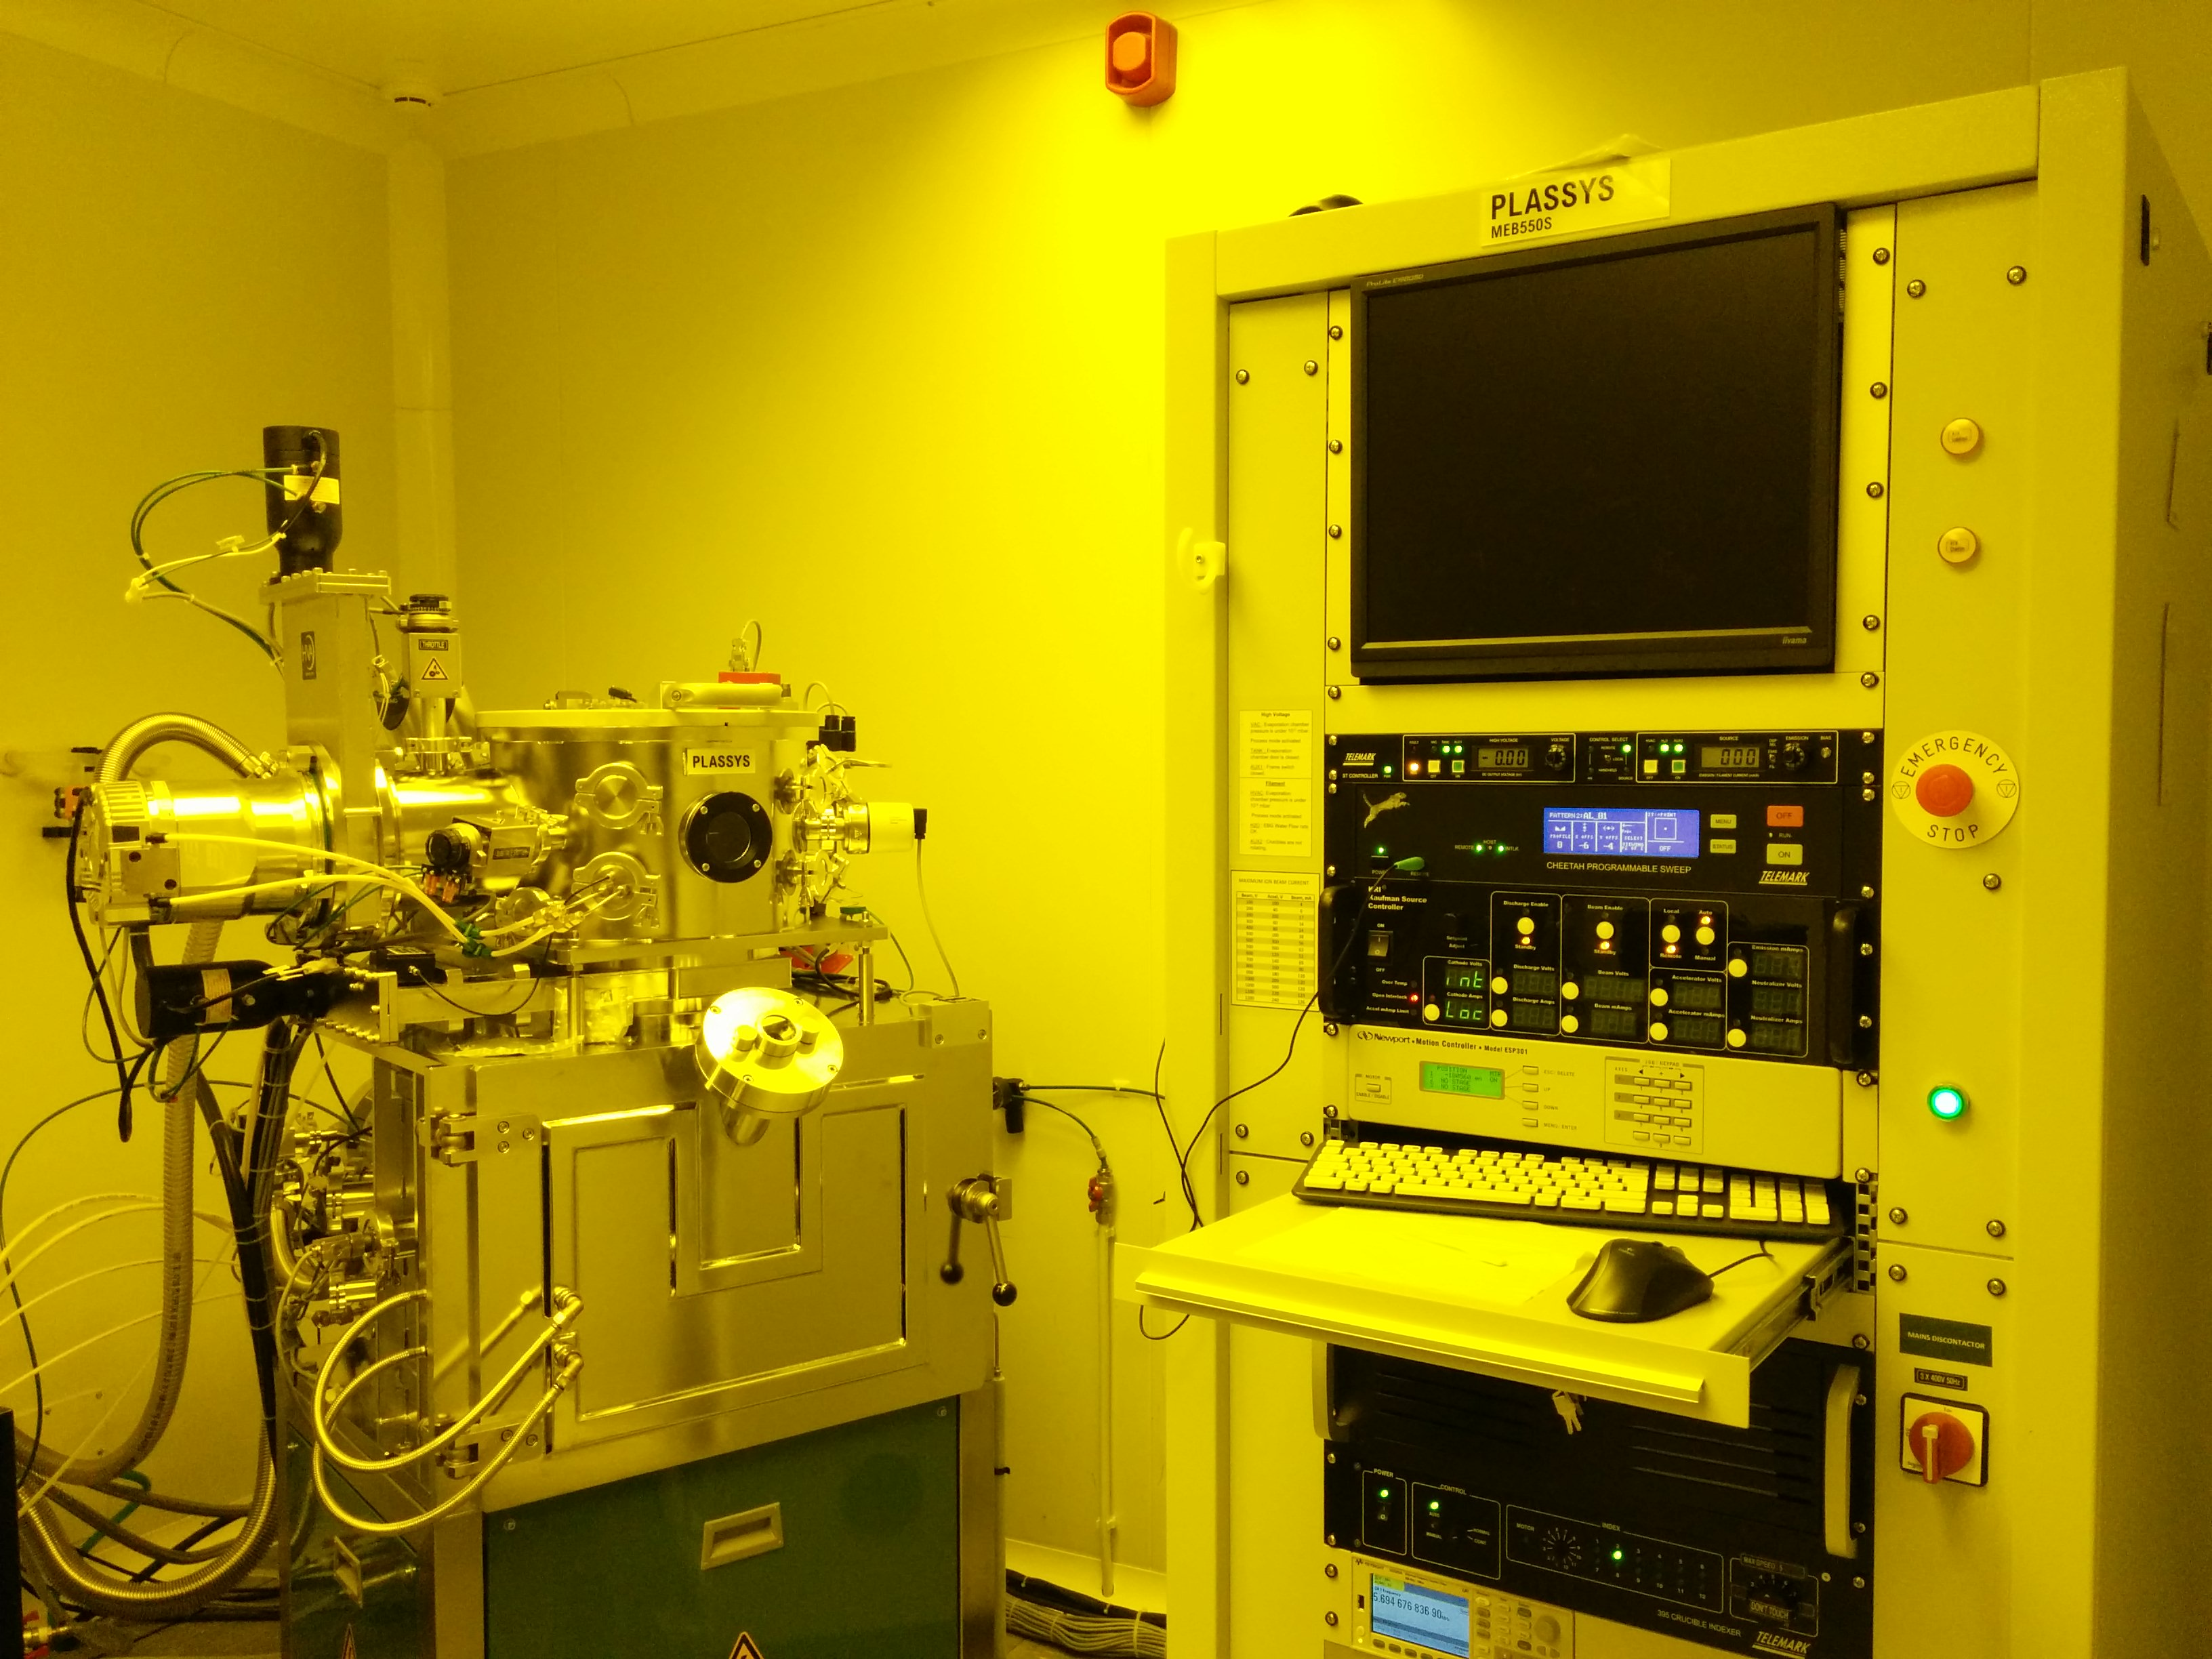
\includegraphics[width=0.6\linewidth]{fig1}
  	\captionof{figure}{MEB 550S}
  \end{center}
\end{minipage}
\begin{minipage}{.49\textwidth}
	\begin{center}
 		 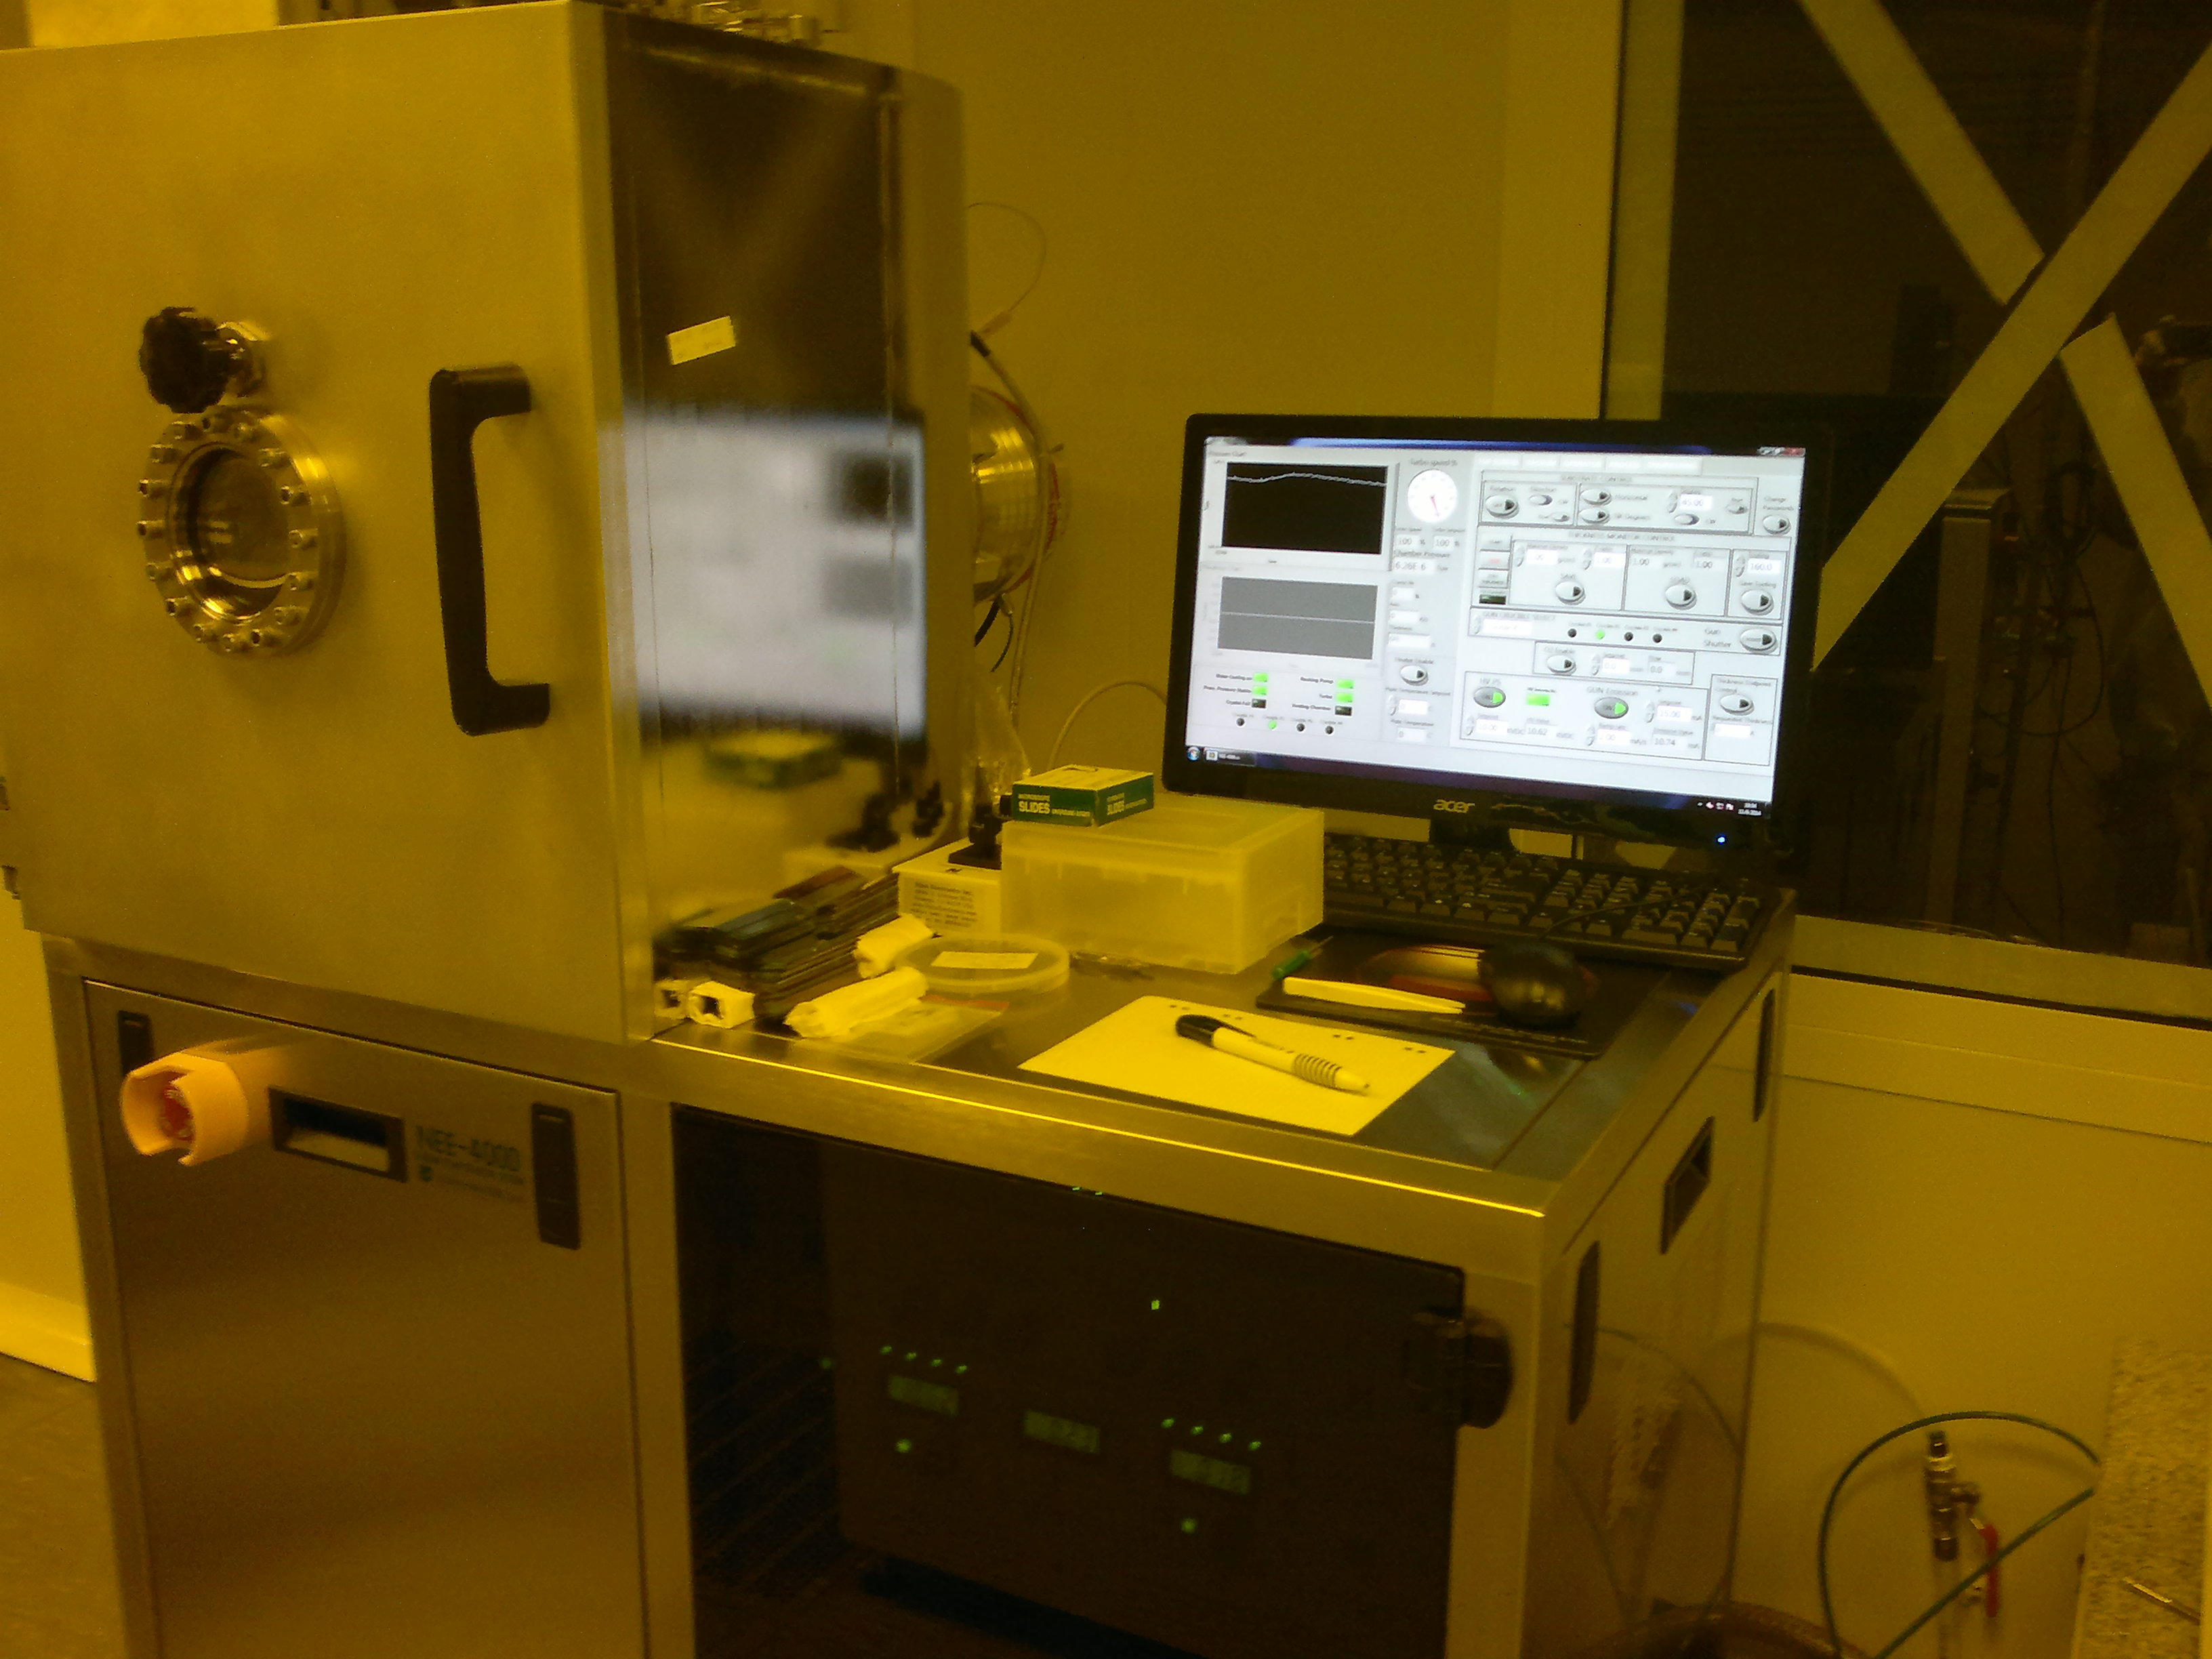
\includegraphics[width=0.6\linewidth]{fig2}
 		 \captionof{figure}{Nanomaster NEE-4000}
  	\end{center}
\end{minipage}

Как было сказано ранее, напыление производилось  с помощью электронно-лучевого испарителя. Кратко обсудим принцип его действия. Сущность электронно-лучевого воздействия состоит в том, что кинетическая энергия электронного пучка превращается в зоне обработки в тепловую. 

\begin{wrapfigure}{l}{0.35 \linewidth} 
	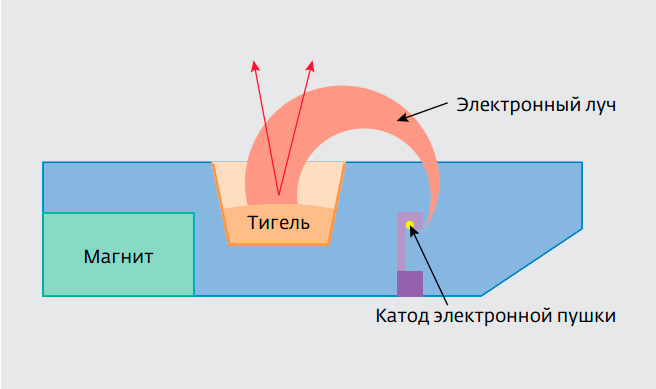
\includegraphics[width=\linewidth]{fig3}
	\caption{Схема электронно-лучевого испарителя}
\end{wrapfigure}

Для формирования потока электронов предназначена электронная пушка, состоящая из вольфрамового термокатода и фокусирующей системы.Эмитируемые электроны проходят эту систему, ускоряются за счет разности потенциалов до 10 кВ между катодом и анодом и формируются в электронный луч. Отклоняющую систему создает магнитное поле, перпендикулярное направлению движения выходящих из фокусирующей системы пушки электронов. Это поле направляет электронный луч в центральную часть водоохлаждаемого тигля, причем в месте падения луча создается локальная зона разогрева и испарения вещества из жидкой фазы. Поток испарившегося материала осаждается в виде тонкой пленки на подложке, которая обычно располагается на определенном расстоянии над испарителем.

\subsection{Нанесение контактов}

\begin{wrapfigure}{l}{0.5 \linewidth} 						    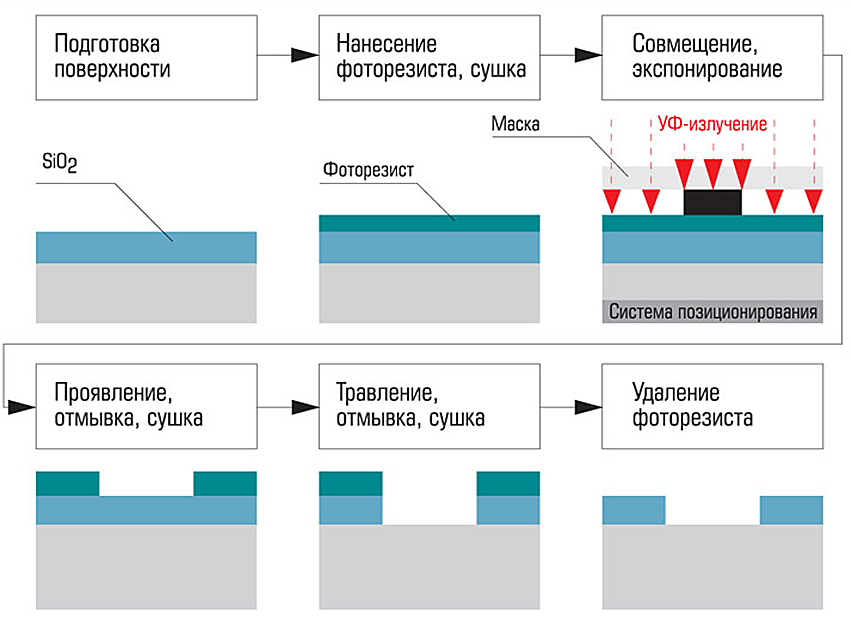
\includegraphics[width=\linewidth]{fig4}
	\caption{Технологический процесс фотолитографии}
\end{wrapfigure}

Для изучения вольтамперной характеристики диода необходимо нанести на него контакты, с помощью которых будет измерена зависимость.

Для нанесения рисунка на пластину pSi используется фотолитография. Сначала на пластину наносится тонкий слой фоточувствительной полимерной пленки (фоторезист) с помощью центрифугирования.

После, фоторезист засвечивается через фотошаблон, содержащий желаемый рисунок, светом видимого или ультрафиолетового диапазона. В результате под действием энергетического воздействия (излучения)
ультрафиолета изменяются свойства резиста.

Далее, при проявлении, части засвеченного фоторезиста удаляются специальной жидкостью -- проявителем.

\section{Теоретические сведения}

\subsection{Зонные диаграммы}
Для объяснения физики процессов, происходящих в полупроводниковых диодах, обратимся к зонным диаграммам. На рис. 1 представлены зонные диаграммы для металла, полупроводника и диэлектрика

\begin{figure}[h!]
	\begin{center}
	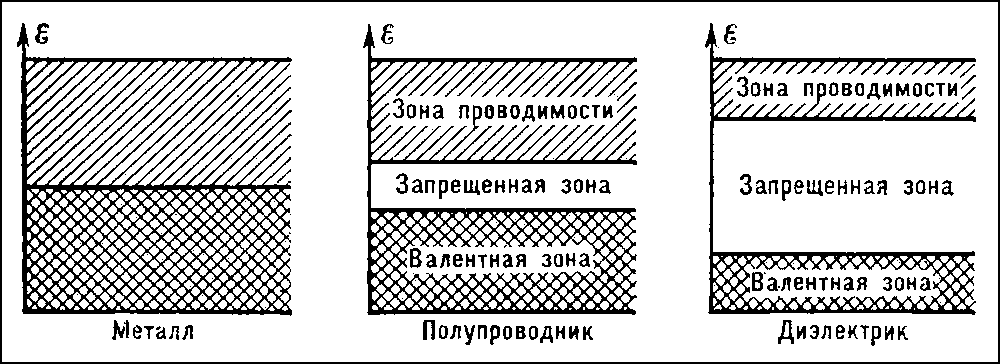
\includegraphics[scale = 0.4]{fig5}
	\caption{Зонные диаграммы металла, полупроводника и диэлектрика}
	\end{center}
\end{figure}

На шкале энергии можно отметить различные зоны и уровни \\
•	Валентная зона – область, состоящая из конечного набора значений энергии (уровней), которые могут занимать электроны.  \\
•	Запрещенная зона – область, в которой не могут находиться электроны. У металла чаще всего нет запрещенной зоны. \\
•	Зона проводимости – область разрешенных энергий, в которой при T = 0 электроны отсутствуют, однако при повышении температуры они могут туда подняться. Уровень вакуума – это верхний край зоны проводимости.  \\

\begin{figure}[h!]
	\begin{center}
	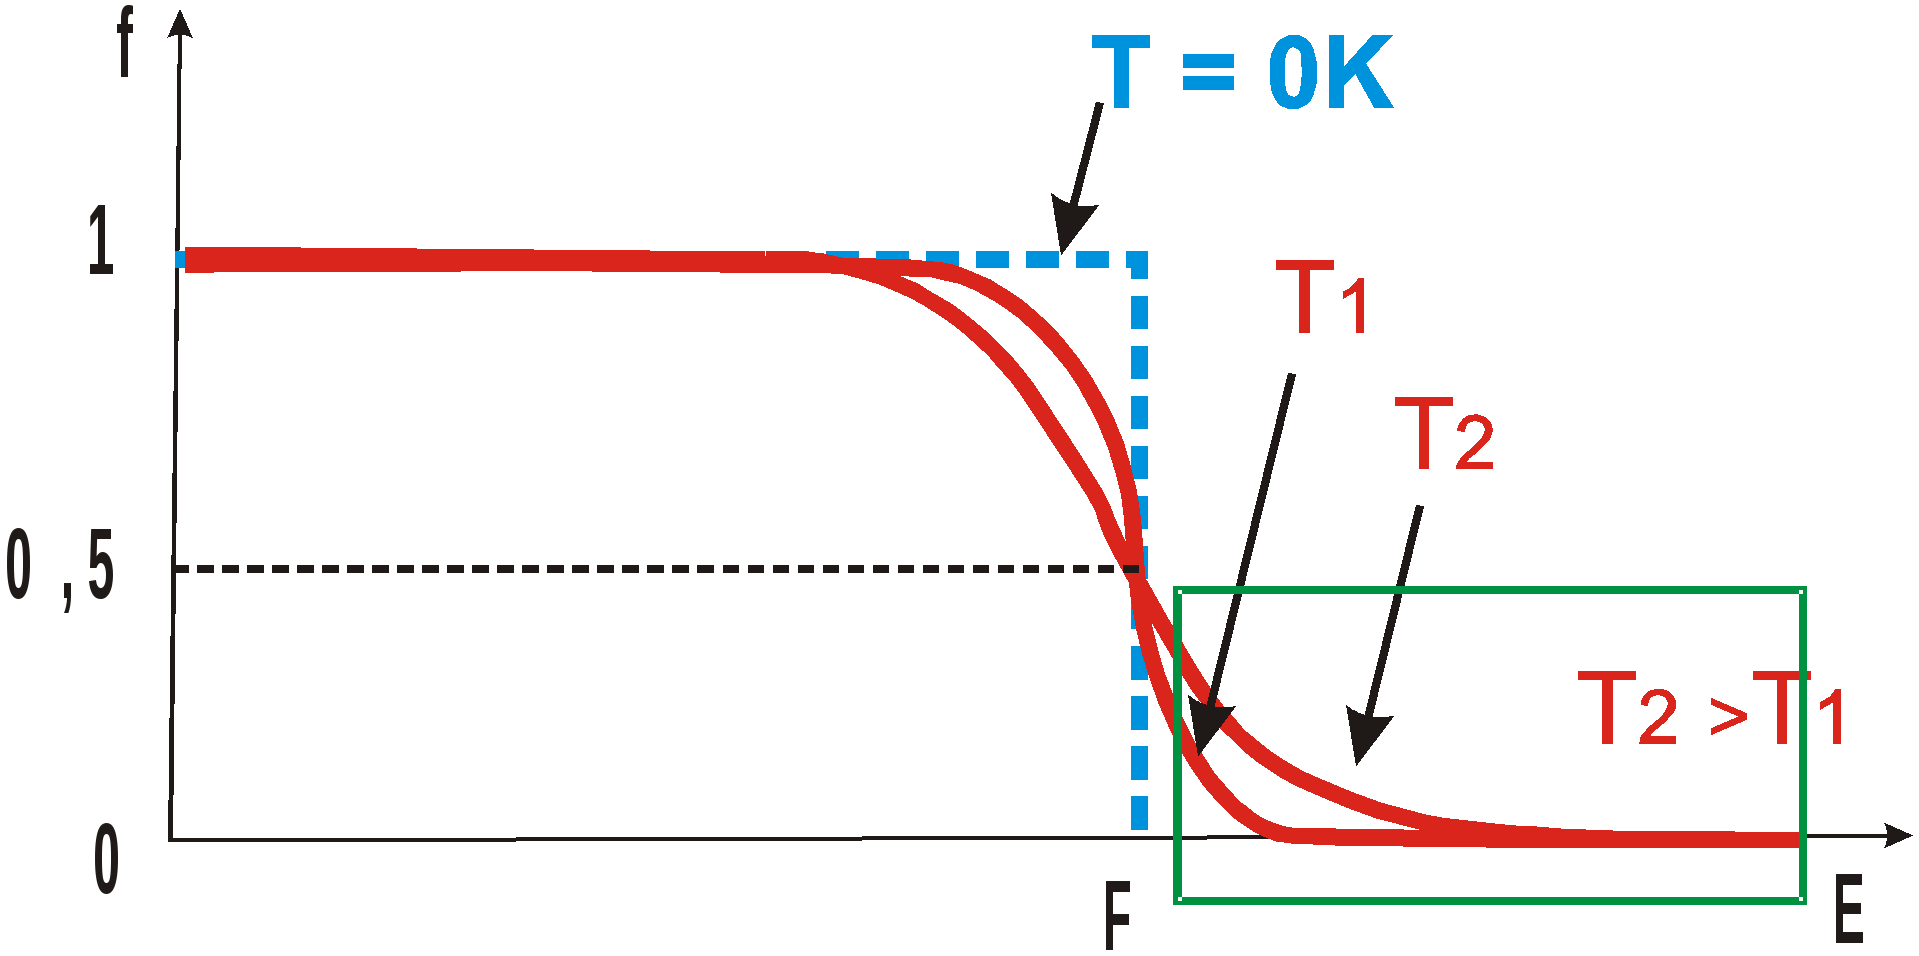
\includegraphics[scale = 0.2]{fig6}
	\caption{График функции распределения Ферми-Дирака}
	\end{center}
\end{figure}

Уровень Ферми – это верхний заполненный электронами металла уровень при Т = 0. Более общее определение основывается на уравнением Ферми-Дирака:

\begin{equation}
f(E) = \frac{1}{1 + \exp(\frac{E-E_F}{kT} Ваня)}
\end{equation}

Из него видно, что уровень Ферми – это уровень энергии, вероятность попадания электрона на который равна 1/2 при любой температуре.

\subsection{Полупроводники p- и n- типа}

Работа выхода - это разность между уровнем вакуума и уровнем Ферми. 

Изменить работу выхода полупроводника можно добавив к нему примесные вещества и тем самым изменив его уровень Ферми. Например, если в кремниевый полупроводник добавить атом Сурьмы имеющий 5 валентных электронов на внешнем уровне, то 4 из них образуют связи с электронами кремния, а оставшийся неспаренный электрон займет так называемый донорный уровень. Донорный уровень находится вблизи дна зоны проводимости, поэтому энергия Ферми полупроводника повысится, а работа выхода соответственно уменьшится. Получится полупроводник n-типа 

\begin{figure}[h!]
	\begin{center}
	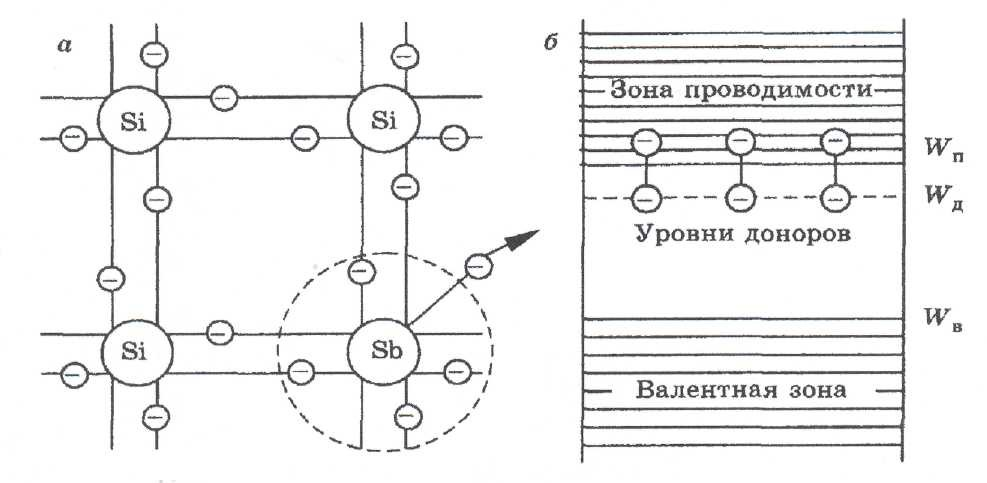
\includegraphics[scale = 0.6]{fig7}
	\caption{Полупроводник n-типа}
	\end{center}
\end{figure}

сли же добавить атом с меньшим чем у кремния числом валентных электронов (напр. Индий), то образуется положительная дырка. Положительные заряды займут акцепторный уровень вблизи верха валентной зоны, за счет чего уровень Ферми понизится, а работа выходы – повысится. Это полупроводник p-типа.

\begin{figure}[h!]
	\begin{center}
	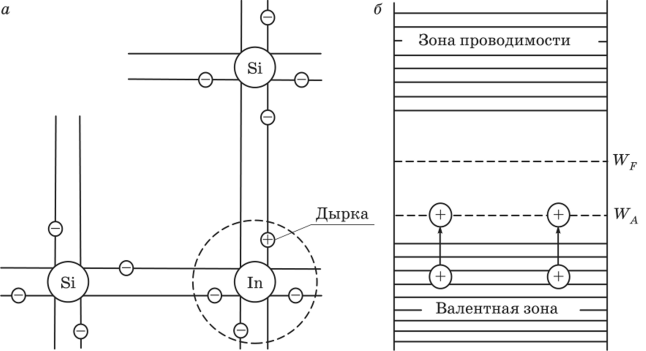
\includegraphics[scale = 0.7]{fig8}
	\caption{Полупроводник p-типа}
	\end{center}
\end{figure}

\subsection{Виды контактов металл-полупроводник}

Диод Шоттки – это металл и полупроводник, приведенные в контакт. Из-за того, что работы выхода металла и полупроводника могут отличаться, в месте контакта будет возникать разность напряжений. 

Выпрямляющий контакт металл -- n-полупроводник может быть реализован, когда работа выхода полупроводника меньше работы выхода металла. В этом случае уровень Ферми металла находится ниже УФ полупроводника и заполненность зоны проводимости полупроводника выше заполненности соответствующих энергетических уровней металла. Поэтому при таком контакте электроны из полупроводника переходят в металл за счёт внутренней термоэлектронной эмиссии. На месте ушедших электронов остаются расположенные в узлах решетки положительные нескомпенсированные ионы донорной примеси, которые формируют в полупроводнике неподвижный объёмный пространственный заряд. Объёмный заряд создаёт в полупроводнике барьерное электрическое поле, направленное из полупроводника в металл. Это запирающее напряжение называется барьером Шоттки.

Уход электронов из полупроводника в металл, сопровождающий процесс выравнивания УФ, снижает их концентрацию в приконтактной области полупроводника. Поскольку концентрация электронов однозначно связана с положением УФ, то её уменьшение вызывает изгиб энергетических зон «вверх» вблизи контакта.

Далее, если подключить к такому устройству источник питания, то  \\
а) разность напряжений, создаваемая внешним источником, будет увеличивать запирающее поле и ток не пойдет \\
б) внешнее поле будет уменьшать барьер и в цепи потечет ток

\begin{minipage}{.49\textwidth}
  \begin{center}
 	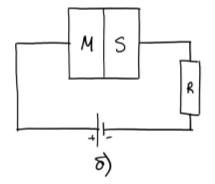
\includegraphics[width=0.6\linewidth]{fig9}
  \end{center}
\end{minipage}
\begin{minipage}{.49\textwidth}
	\begin{center}
 		 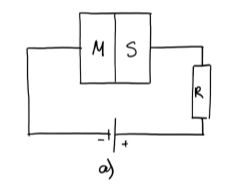
\includegraphics[width=0.6\linewidth]{fig10}
  	\end{center}
\end{minipage}

Выпрямляющий контакт металл -- p-полупроводник может быть реализован, когда работа выхода полупроводника больше работы выхода металла. Поэтому направление термоэмиссионных потоков электронов первоначально тоже будет обратным – из металла в полупроводник. В результате этого в приповерхностном слое увеличится концентрация нескомпенсированных ионов, которые формируют отрицательный объемный заряд. Этот заряд создаст барьерное электрическое поле E направленное из металла в  полупроводник.

\begin{figure}[h!]
	\begin{center}
	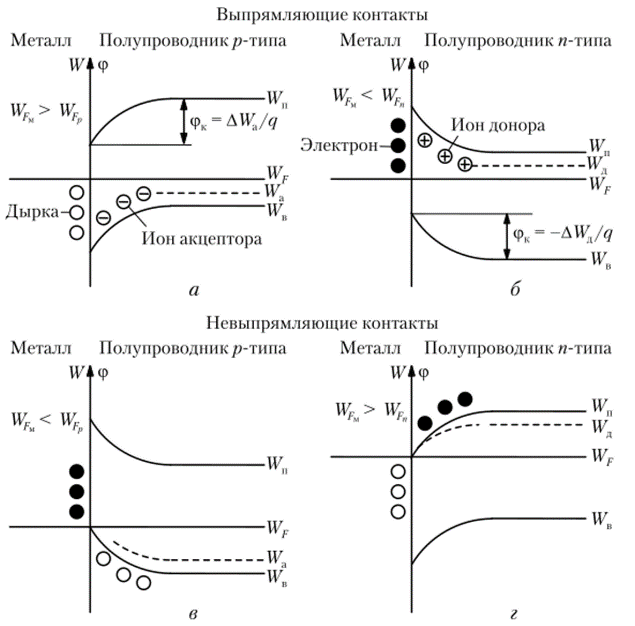
\includegraphics[scale = 0.5]{fig11}
	\caption{Выпрямляющий и омический контакт металла с полупроводником}
	\end{center}
\end{figure}

Омический контакт металл -- n-полупроводник (рис. 7б) может быть реализован, когда работа выхода полупроводника больше работы выхода металла. При таком контакте электроны из металла переходят в полупроводник, значит их концентрация в нем увеличивается, а в металле остаются нескомпенсированные положительные ионы – возникает поле, направленное из металла в полупроводник. Контакт обогащается электронами.

Аналогично . при формировании контакта металл – р-полупроводник, электроны из полупроводника уходят в металл - в контакте действует электрическое поле, направленное из полупроводника в металл. Контакт обогащается ОНЗ – дырками

Таким образом, характерной особенностью невыпрямляющих контактов является наличие слоёв, обогащённых основными носителями заряда. Это означает, что в отличие от выпрямляющих контактов, для которых характерно наличие обеднённых слоёв, сопротивление контакта определяется не барьером, а нейтральным слоем полупроводника. Значит, оно не зависит от величины приложенного напряжения. Кроме того, если за счёт выбора металла, работы выхода полупроводника и металла будут близки, то высота барьера будет минимальной. Контакт с минимальной высотой барьера будет иметь большой ток насыщения, значит, малое сопротивление для прямого и обратного смещения, т.е. будет омическим. ВАХи обоих контактов приведены на рисунке

\begin{figure}[h!]
	\begin{center}
	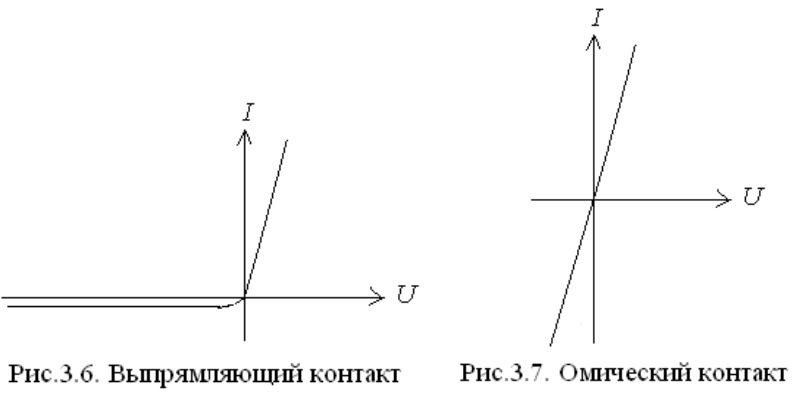
\includegraphics[scale = 0.5]{fig12}
	\caption{ВАХ выпрямляющего и омического контактов}
	\end{center}
\end{figure}

\newpage

\section{Измерение вольтамперной характеристики}

Снятие ВАХ проводилось с готового диода. На зонд, приведенный в
контакт с поверхностью диода, подавался потенциал и проводились измерения сопротивления и силы тока. По снятым данным построим графики зависимости тока на диоде от напряжения на нем.

\begin{figure}[h!]
	\begin{center}
	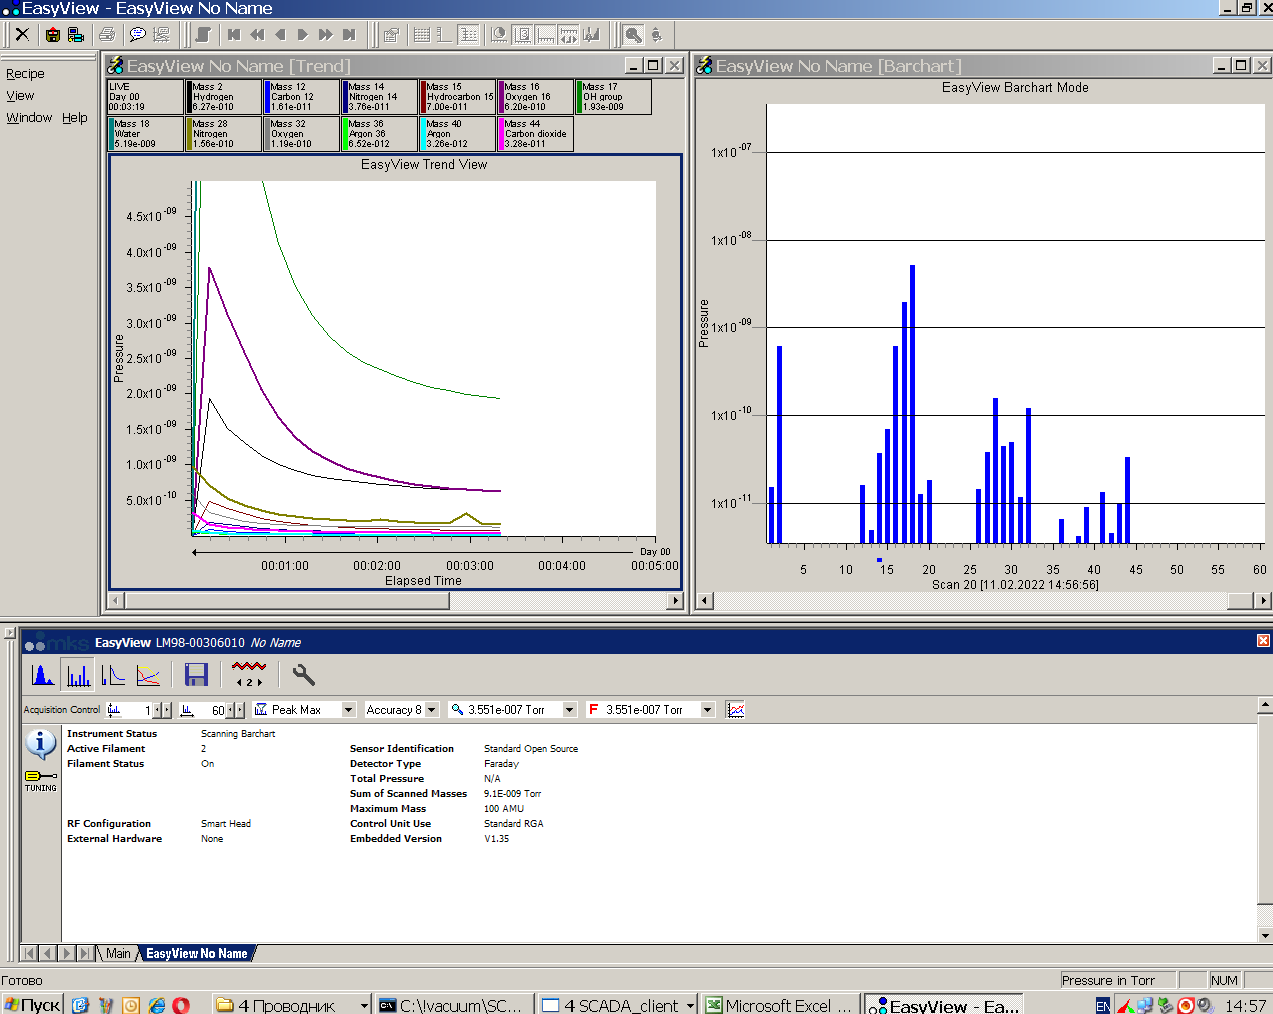
\includegraphics[scale = 0.4]{graph1}
\caption{вольтамперная характеристика омического контакта (Au-pSi)}
	\end{center}
\end{figure}

\begin{figure}[h!]
	\begin{center}	
	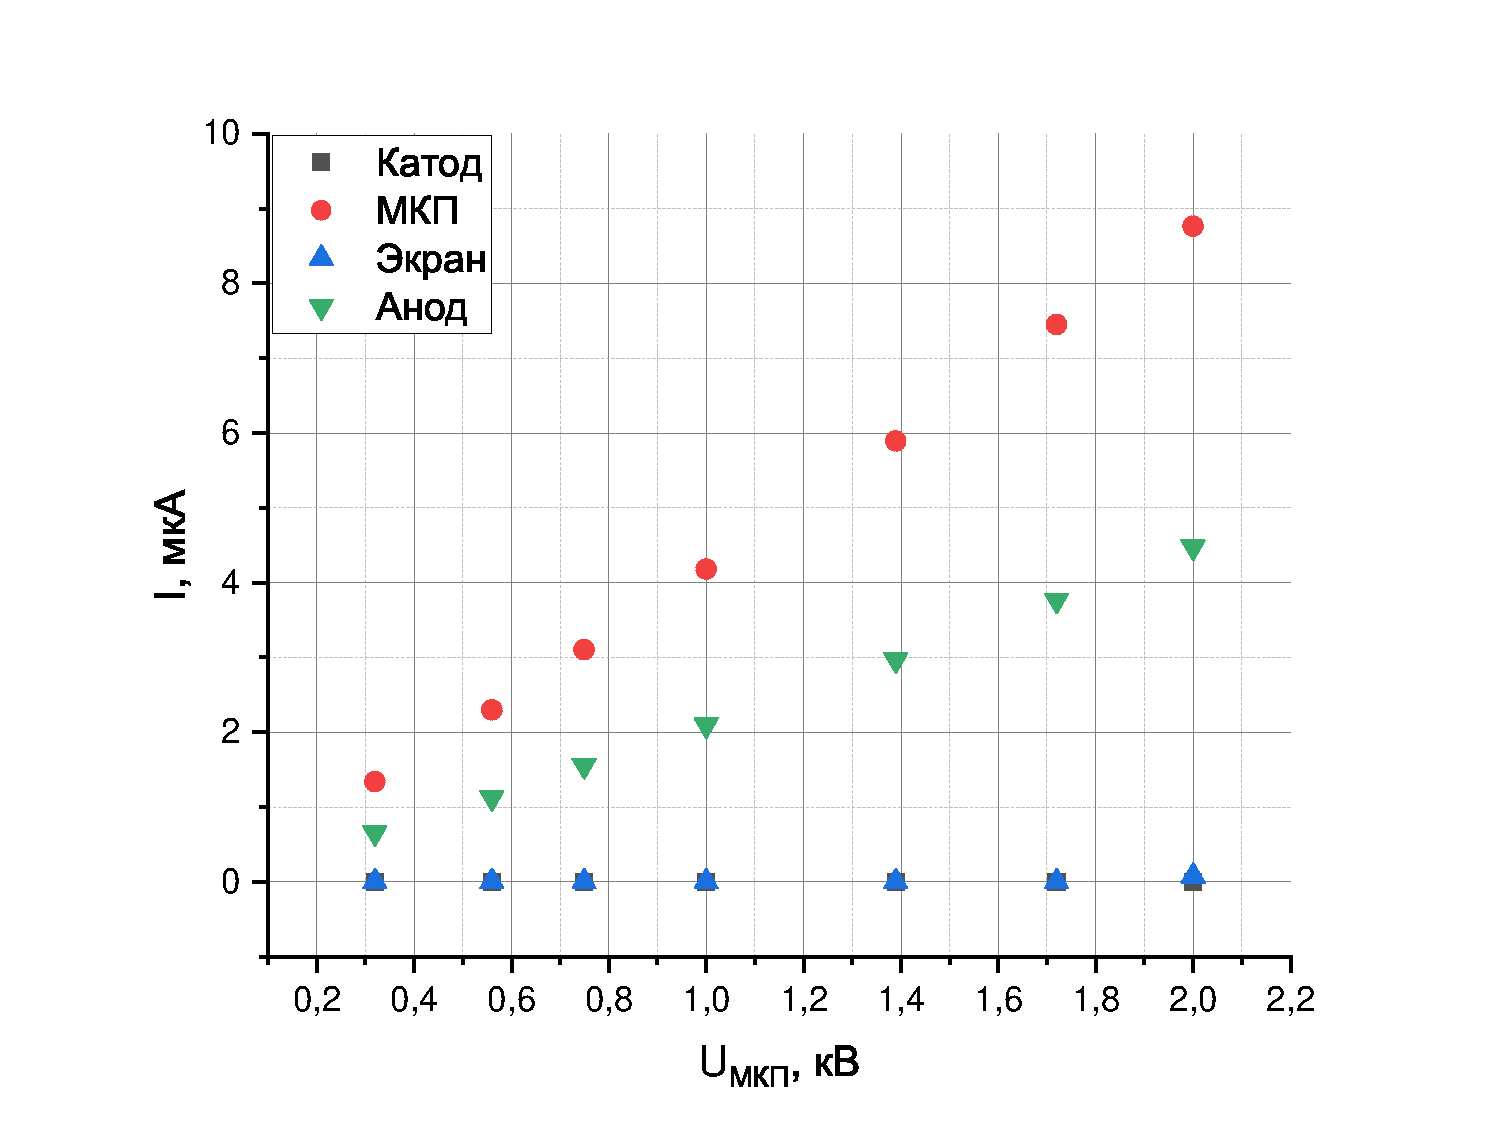
\includegraphics[scale = 0.4]{graph2}
\caption{вольтамперная характеристика диода Шоттки}
	\end{center}
\end{figure}

Из графиков видно, что полученный омический имеет достаточно большое сопротивление ($\sim 10^3 \ Ом$) и зависимость I(U) не является линейной на диапазоне измерений.


\section{Выводы}

1.В результате работы, были получены представления о принципах работы диода Шоттки и методах его изготовления. \\
2.Также были получены зависимости I(U) для диода Шоттки (Al-pSi) и омического контакта (Au-pSi)	




\end{document}